
%% CLASS MANUAL FOUND IN http://blog.poormansmath.net/latex-class-for-lecture-notes/ %%
%% CLASS AUTHOR Stefano Maggiolo %%

%%%%%%%%%%%%%%%  TITLE PAGE  %%%%%%%%%%%%%%%%%%%
\documentclass[english,course]{Notes}
\title{Algorithms \& Data Structures}
\subject{CS}
\author{Joao Almeida-Domingues}
\email{2334590D@student.gla.ac.uk}
\speaker{Dr Michele Sevegnani}
\date{14}{01}{2020}
\dateend{25}{03}{2020}
\place{University of Glasgow}

\graphicspath{{assets/}}
%%%%%%%%%%%% BIB CONFIG %%%%%%%%%%%%%%%
\usepackage[backend=biber, style=reading, citestyle=numeric]{biblatex}

\bibliography{ADT} %add bib file name

%%%%%%%%%%% LAYOUT  %%%%%%%%%%%%%%%

\renewcommand{\abstractname}{\vspace{3\baselineskip}} %hack to remove abstract


%%%%%%%%%%%%%%%%%%%%%%%%%%%%%%%%

%%%%%%%%%%%%%% KEEP HERE (conflict when in class) %%%%%%%%%%%%%%%%%%%%

 %%%%%MATRICES

    \let\mat=\spalignmat
    \let\amat=\spalignaugmat
    \let\vec=\spalignvector

%%%%%% row ops
    \newcommand\ro[2]{\xrightarrow[#2]{#1}}
%%%%%%%%%%%%%%%%%%%%%%%%%%%%%%%%%%%%%%%%%%%%%%%%%%%%%

%%%%%%%%%%%%%  PACKAGES (NOT INCLUDED IN CLASS) %%%%%%%%%%%%%%
\usepackage[delims={[]}]{spalign}

%%%%%%%%%%%%%%%% ALGORITHM TEMPLATE %%%%%%%%%%%%%%%%%%%%

%\begin{algorithm}[H]
%\SetAlgoLined\KwData{this text}
%\KwResult{how to write algorithm with \LaTeX2e }initialization\;
%\While{not at end of this document}
%	{read current\;\eIf{understand}{go to next section\;current section becomes this one\;}{go back to the beginning of current section\;}}
%	\caption{How to write algorithms}
%\end{algorithm}

%%%%%%%%%%%%%%%%%%%%%%%%%%%%%%%%%%%%%%%%%%%%%%%%%%%%%

\begin{document}

%%%%%%%%%%%%%%  DISCLAIMER  %%%%%%%%%%%%%%%%%%%%%

\begin{abstract}
	\par{These lecture notes were collated by me from a mixture of sources , the two main sources being the lecture notes provided by the lecturer and the
content presented in-lecture. All other referenced material (if used) can be found in the \ita{Bibliography} and \ita{References} sections.}
	\par{The primary goal of these notes is to function as a succinct but comprehensive revision aid, hence if you came by them via a search engine , please note
that they're not intended to be a reflection of the quality of the materials referenced or the content lectured.}
	\par{Lastly, with regards to formatting, the pdf doc was typeset in \LaTeX , using a modified version of Stefano Maggiolo's \href{http://blog.poormansmath.net/
latex-class-for-lecture-notes/}{\underline{\textcolor{blue}{class}}}}
\end{abstract}
\newpage

%%%%%%%%%%%%% LECTURES %%%%%%%%%%%%%%%%%%%%%%%
\lstset{language=Java}
%\section{Analysis Techniques}

\key{running time}{experimental analysis}{theoretical analysis}{primitive operations}{growth rate of running time}{Big-Oh}

		\defn{Data Structure}{is a systematic way of organising and accessing data}

		\defn{Algorithm}{is a step-by-step procedure for performing some task in a finite amount of data}

		\defn{Running Time}{is the amount of time it takes an algorithm to execute in full}

		\par{The main criteria used to compare different algorithms are running time and memory usage. In general the running time of an algorithm increases with the
		input size, and may vary depending on the hardware and software environments on which it is run. When comparing algorithms one aims to control those variables
		and express a relation between their run times and inputs via some function}

\subsection{Experimental Analysis vs Theoretical Analysis}

		\par{One way to study the efficiency of an algorithm is to run an empirical study. The dependent and independent variables are set, several trials are run a
		with appropriate inputs and then a statistical analysis is carried out on the output of the experiments.}

		%INSERT PLOT p.141

		%\caption{The plot above compares two algorithms for string concatenation in Java.}

		\par{\mymarginpar{Drawbacks}Though the experiment itself is relatively straightforward to run (once the algorithm is implemented), the analysis can be quite quite complicated to
		perform. Especially given that it can be hard to know which inputs are appropriate to use and , more importantly , given that fully implementing a complex algorithm is hard
		work and time-consuming. Hence, if possible a higher-level analysis is performed, if an algorithm can be deemed to be inferior by application of theoretical
		methods then no experimental analysis is required}


\par{So, when developing theoretical methods of analysis one's goal is to overcome the drawbacks mentioned above in order to achieve the following:}

\begin{enumerate}
	\item System Independence
	\item Input Coverage
	\item High-Level Description
\end{enumerate}


\defn{Primitive Operations}{are \ita{low-level} instructions with constant execution time (e.g. variable assignment, function call)}

\par{In order to express running time as a function of input size we use primitive operations, which are identifiable from abstract implementations (like
pseudocode) and taken to have a constant time of completion. In this way, one can compare the total number $t$ of ops for a given implementation, since by
assuming a constant time for all ops one can assume that the total running time will be \ita{proportional} to $t$}

\par{Ideally the average of all possible inputs would be used to characterize a given algorithm. However,finding the average often involves finding an
		appropriate distribution for the sample inputs. Hence, we characterize it instead in terms of its \ita{worst case} input which is far easier to
		identify. }
\rem{Another advantage is that minimising for the worst case by definition implies that we're optimising the running time for all other possible
inputs}

\subsection{Common Functions}

\par{This relation between input and running time is often expressed in terms of one of the following 7 functions}

\subsubsection{Constant}

	\par{The simplest function of them all is the constant function which simply
	assigns a given constant $c$ to any input $n$ . It is particularly useful,
	since it allows us to express the \ita{number of steps} needed to perform a basic
	operation}

	$$f(n) = c , \forall n \in \text{ input set }$$

	\rem{The essential constant functions if $g(n) = 1$ given that we can
	express any other constant function in the form $g(n)f(n)$}

\subsubsection{Logarithm}

	\par{The logarithmic function, in particular $\log_2$ , pops up all the
	time. A logarithmic runtime is characterized by larger differences in
	runtime for smaller inputs, with a significant decrease for larger inputs.}

	\defn{ceiling (of $x$)}{the smallest integer greater than x}

	\nota{$\lceil x \rceil$}

	\par{We can think of the ceiling function as an approximation of x. We can
			use it in a similar manner to approximate any given algorithm. By
			definition $\log_b(x)$ is just the power to which $b$ has to be
			raised to give $x$. Hence, we define $\lceil\log_b x\rceil$ as the
	smallest number for which $b$ has to be raised so that it includes $x$. So,
	we can divide repeatedly divide $x$ by $b$ until we get a number less or
	equal to 1}

	\ex{ $\lceil\log_{2}12\rceil = 4$ since $2^3 < 12 < 2^4$}

\subsubsection{Linear}

	\par{The linear function assigns the input to itself. It is useful to
	characterize single basic operations on $n$ elements}

	$$f(n) = n$$

\subsubsection{N-Log-N}

	\par{For any given input $n$ it assigns $n$ times $\log(n)$}

	$$f(n) = n\log(n)$$

\subsection{Quadratic}

	\par{The quadratic function appears primarily in algorithms with nested
			loops, since the inner loop performs an operation $n$ times and the
	outer loop will repeat each loop a \ita{linear} number of times}

	$$f(n) = n^2$$

\subsubsection{Polynomials}

\par{A more general class which subsumes the quadratic ($d=2$), linear ($d=1$)
		and constant ($d=0$) functions, where $d$ is the degree of the
		polynomial which corresponds to the largest exponent in the polynomial
		expression. In general, polynomials with lower degrees have better
running times}

$$f(n) = \sum_{i=0}^{d} a_{i}n^{i}$$

\subsubsection{Exponential}

	\par{Exponential time polynomials are generally the worst-case running time
			for an algorithm, since they grow very rapidly. As an example, take
			a loop which doubles the number of operations it performs with every
			iteration. Then, the total number of operations it performs will be
	$2^n$}


\subsection{Growth Rates}


	\par{If we take $f(n)$ to be the function which gives the total number of
			operations in the \ita{worst-case}, and $a\;z$ to be the time taken
			by the fastest and slowest primitive op , respectively. Then, the
			worst-case running time $T(n)$ for the algorithm is bounded by the two
	linear functions $af(n);zf(n)$ , i.e}

	$$af(n) \leq T(n) \leq bf(n)$$

	\par{Note that the growth rate of the worst-case running time is an
			intrinsic property of the algorithm which is not affected by by
	hardware or software environments. These factors affect $T(n)$ by a constant
	factor. Hence, when running an asymptotic analysis one can \textbf{disregard} constant
	and lower-degree terms}

	\rem{Ideally we want operations on data structures to run in times
			proportional to the constant or log functions, and algorithms to run
	in linear or n-log-n}

	\defn{Asymptotic Analysis}{analysing how the running time of an algorithm
			increases with the size of the input \ita{in the limit}, as the size
	of the input increases with the bound}

	\begin{figure}[H]
		\begin{center}
		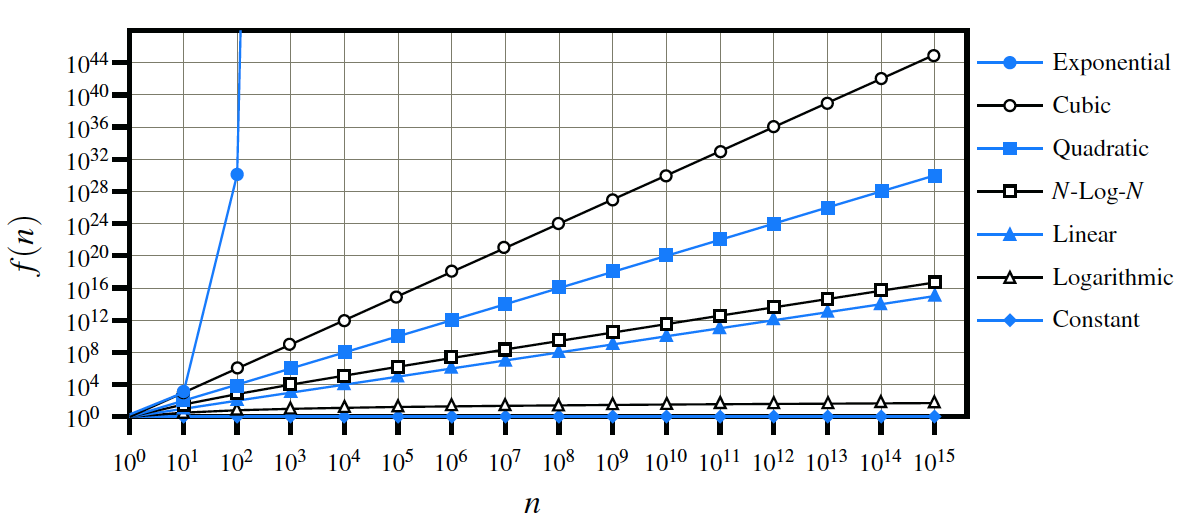
\includegraphics[width=\textwidth]{growth.png}
		\end{center}
	\end{figure}

\subsection{Big-Oh Notation}



		\defn{Big-Oh Notation}{we say that \ita{"$f(n)$ is big-Oh of $g(n)$"} if
		$\exists c \in \real s.t f(n) \leq cg(n)$ , for $n \geq n_0$}

		\notation{$f(n) is O\left(g(n)\right)$}
		\par{In essence we make use of the fact that growth run time is not affected by
				constant factors, and encode this into function notation. In effect
				bounding the function after a given input size $n_0$ by another
		function ; i.e $f(x)$ is strictly less than or equal to $g(x)$ up to to a
		constant factor and in the \ita{asymptotic sense}. Hence, we can use $g(x)$ to
		approximate/characterize $f(x)$}

		\par{We want this relation to be expressed in the simplest terms possible. Obviously it is easy to find such a function if one aims for the moon, i.e
				clearly $3n^2 + 2$ is $O(n^{10})$ this is however not very useful.
				Instead, simplifying the first expression by getting read of constant
				factors , we see that we can be sure that it is for sure $O(n^2) < O(n^{10})$,
		which is therefore a better approximation}

		\rem{We want the \ita{simplest} expression of the class of bounding functions
				($n^{2}$ Vs $4n^{2}$) and the \ita{smallest} possible class ($n^{2}$ Vs
		$n^{10}$)}

		\proposition{}{For any polynomial $p(n)$ of degree $d$ , $p(n) \in
		O\left(n^d\right)$}

		\proposition{}{$T_1(n) \in O(f(n)) , T_2(n) \in O(g(n)) \implies T_1(n)
		+ T_2(n) \in O(max(f(n),g(n)))$}

		\proposition{}{$T_{1}(n) \in O(f(n))$ and $T_{2}(n) \in O(g(n)) \implies
		T_{1}(n)T_{2}(n) = O(f(n)g(n))$}

		\proof{$T_{1}T_{2} = klf(n)g(n)$ , for constants $k,l$ . Hence, ignoring
		the constants we have the expected result}

		\prop{$T(n) = (\log n)^k \implies T(n) = O(n)$}

		\proof{$$T(n) \in O(f(n)) \iff \lim_{n\to\infty}(T(n) / f(n)) = 0)$$
		 \par{By \ita{L'Hopital's},  }$$lim_{n\to\infty}(f(n) / g(n)) =
				lim_{n\to\infty}(f\prime(n) / g\prime(n))$$

				\par{Take $f(n) = (\log n)^{k+1}$ and $g(n) = n$. Then, by
						induction on $k$ , $$(\log n)^1 = \log n \in O(n) \text{ and } (\log n)^k \in O(n)$$}

				\par{Hence, $$\lim_{n\to\infty}\left(\frac{(\log n)^{k+1}}{n}\right) = 0$$
						$$\lim_{n\to\infty}\left(\frac{(\log n)^{k+1}}{n}\right) =
				\lim_{n\to\infty}\left(\frac{(k+1)(\log n)^k}{n}\right) = 0$$}

				\par{Therefore, the result follows by induction}
		}
\subsection{Big-Omega \& Big-Theta}

		\defn{$\Omega\left(n\right)$}{$f(n) \geq cg(n)$}

		\defn{$\Theta\left(n\right)$}{$c\prime g(n) \leq f(n) \leq c\prime\prime g(n)$}

		\par{Similarly to $O\left(n\right)$ , these provide upper and upper+lower bounds
		respectively}


		\begin{figure}[H]
		\begin{center}
				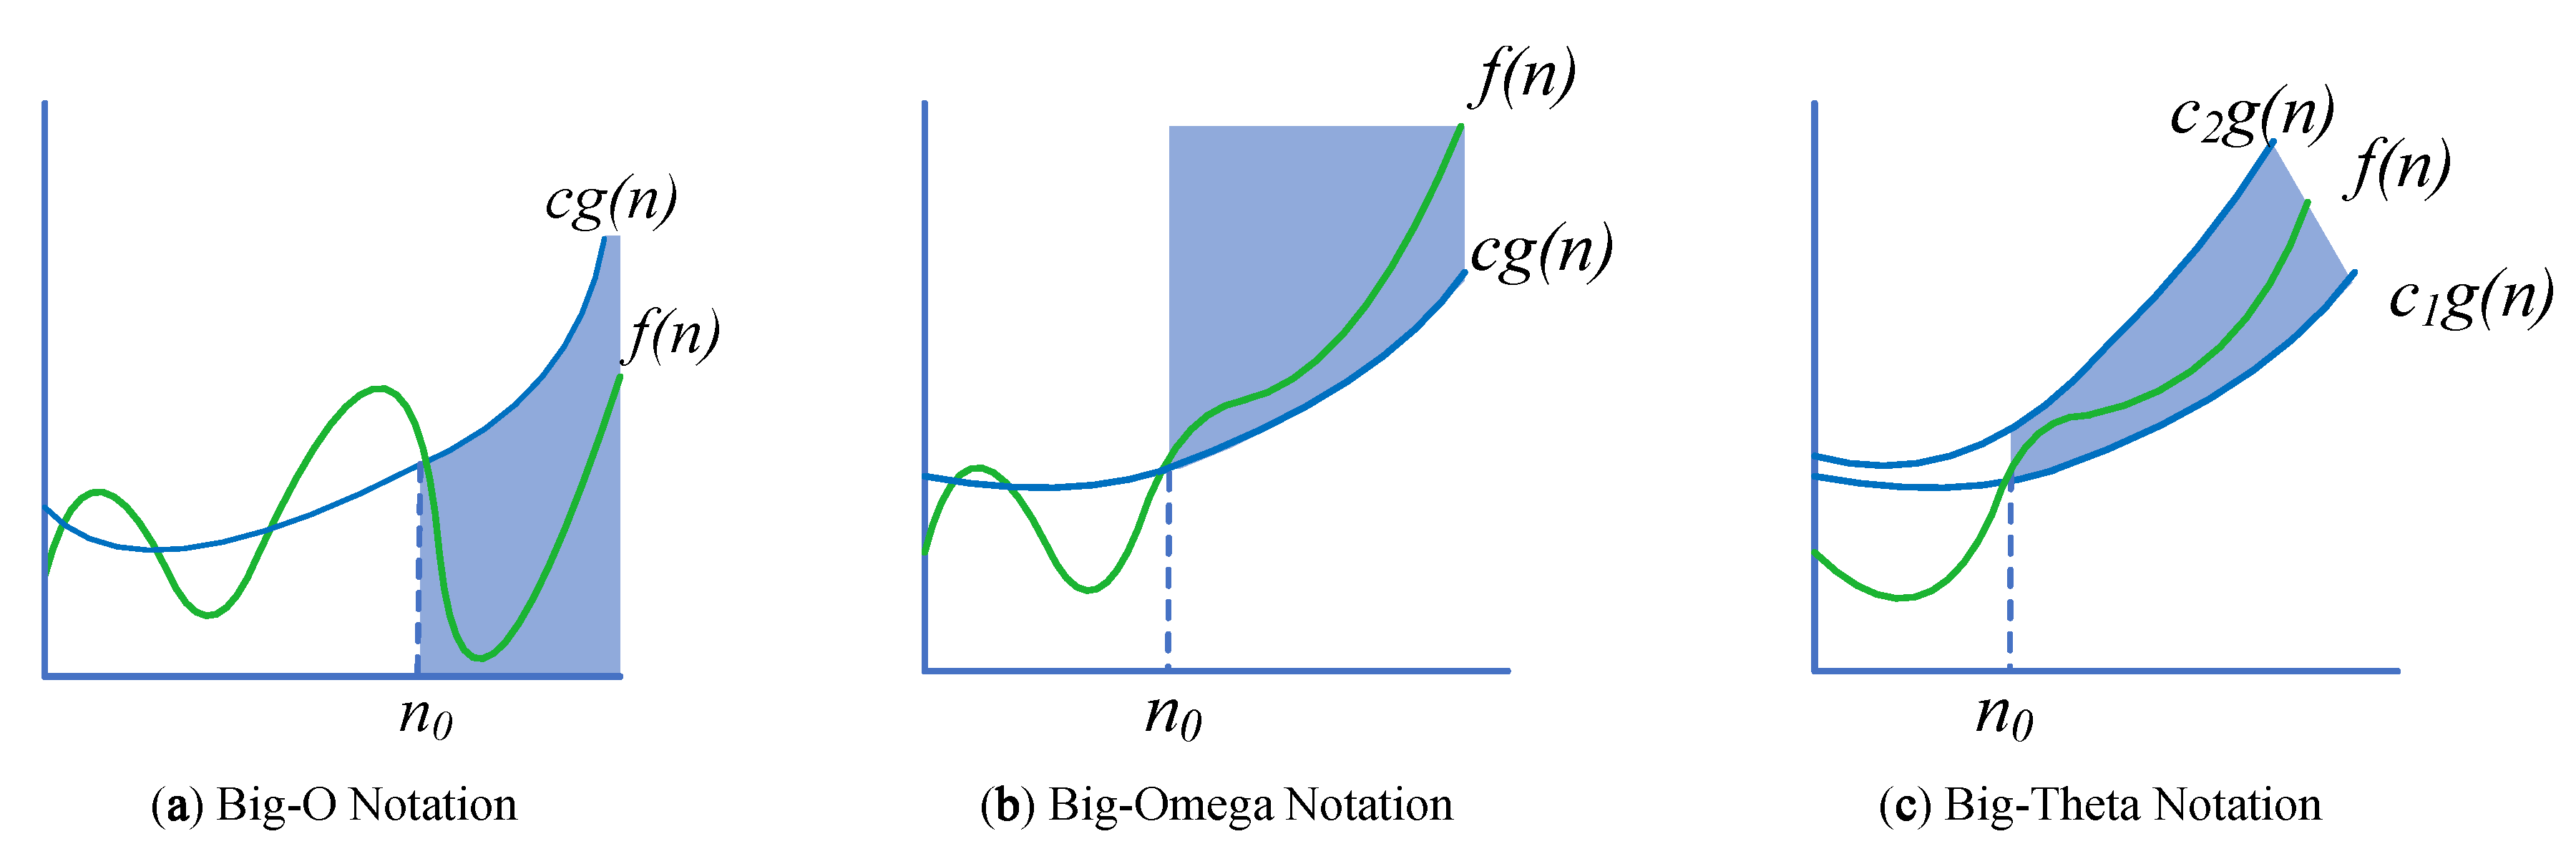
\includegraphics[width=\textwidth]{big.png}
		\caption{Asymptotic Notation
		\url{shorturl.at/xAFQ1}}
		\end{center}
		\end{figure}
\subsection{Little-oh}

\defn{$o(g(n))$}{$\lim_{n\to\infty}\frac{f(n)}{g(n)} = 0}

\par{We say that $f(x)$ is $o(g(x))$ if $g(x)$ grows much faster than $f(x)$,
i.e. if $f(n)$ is $O(g(n))$ and $f(n)$ is not $\Omega(g(n))$}


\subsection{Computing Running Times}

	\par{The following, follows from the propositions above}

	\begin{enumerate}
			\item\textbf{Loops : } at most the running time of its contents times
					the number of iterations
			\item\textbf{Nested Loops : } it should be analysed inside out. Take
					the runtime of the expression and multiply it by the product
					of of the sizes of all the loops
			\item\textbf{Consecutive Statements : } add
			\item\textbf{If-then-else : } at most the time of the test condition
					with the maximum of the running times of the two branches
	\end{enumerate}

	\example{

		\begin{lstlisting}
			sum = 0;
			for (i=1; i<=n; i++)
				sum += n;
		\end{lstlisting}



	\par{See more examples
	\href{https://opendsa-server.cs.vt.edu/ODSA/Books/CS2/html/AnalProgram.html}{here}}
	}
\subsubsection{Analysis of Insertion-Sort}
	\example{Insertion-Sort \\
	\begin{algorithm}[H]
	\DontPrintSemicolon
	\SetAlgoLined\KwData{Array of integers : A}
	\SetKwFunction{KwFn}{Insert}
	\KwResult{Permutation of A such that A[0] $\leq$ A[1] $\leq \dots$ A[n-1] }
	\KwFn{A}\\
	\For{$j=1$ \KwTo $n-1$}{\tcc*[r]{$n$}
	    key := A[j]\tcc*[r]{$n-1$}\;
	    i := j-1\tcc*[r]{$n-1$}\;
	    \While{$i \geq 0$ {\bf and} $A[i] > key$}{\tcc*[r]{$\sum_{1}^{n-1}t_j$}
	        A[i+1] := A[i]\tcc*[r]{$\sum_{1}^{n-1}(t_{j}-1)$}\;
	        i := i-1\tcc*[r]{$\sum_{1}^{n-1}(t_{j}-1)$}\;
	    }
	    A[i+1] := key\tcc*[r]{$n-1$}\;
	}
		\caption{Insertion-Sort}
	\end{algorithm}
	\vspace{3mm}
	\par{Hence, summing the individual operations $$T(n) = n + (n-1) + (n-1)  + \sum_{1}^{n-1}t_{j} + \sum_{1}^{n-1}(t_{j}-1) + \sum_{1}^{n-1}(t_{j}-1) + (n-1)$$ }

	\par{\textbf{Best Case:} $A$ is already sorted , which means that the while loop is never executed and $t_j = 1$. Hence,
	$$ T(n) = n + (n-1) + (n-1)  + (n-1) + 0 + 0 + (n-1) = O(n)$$}

	\par{\textbf{Worst Case:} At every iteration we shift $j$ elements : $t_j = j$. So,
		$$\sum_{1}^{n-1}t_{j} = \sum_{1}^{n-1}j = \frac{n(n-1)}{2} = O(n^2)$$
		$$\sum_{1}^{n-1}t_{j}-1 = \sum_{1}^{n-1}(j-1) = \frac{n(n-1)}{2} - (n-1) = O(n^2)$$
		Hence,
		$$T(n) = n + (n-1) + (n-1)  + O(n^2) + O(n^2) + O(n^2) + (n-1) = O(^2)$$
	}
}

%
\section{Recursive Algorithms}

\key{recursion traces}{linear recursion}{binary recursion}{tail
recursion}{recursion trees}{incremental algorithms}{divide-and-conquer
algorithms}{merge-sort}

\defn{Recursive Function}{is a function which refers to itself in its
definition}

\par{A classical example of a recursive faction is the factorial function, which
calls itself always with an argument decreased by one in each call, until the
\ita{base case} 1 is reached.}
\par{All recursive definitions share these 2 properties, i.e they all have a
base case which tells us when to stop calling, and they must reduce the size of
the data set with each call}

\subsection{Recursion Trace}

\par{A recursion trace allows us to visually trace the execution of recursive
algorithms. We draw a box for each call with an arrow pointing downwards
connected to the next call, and an arrow pointing upwards with the returning
value of that call}

\ex{\vphantom{.\\}
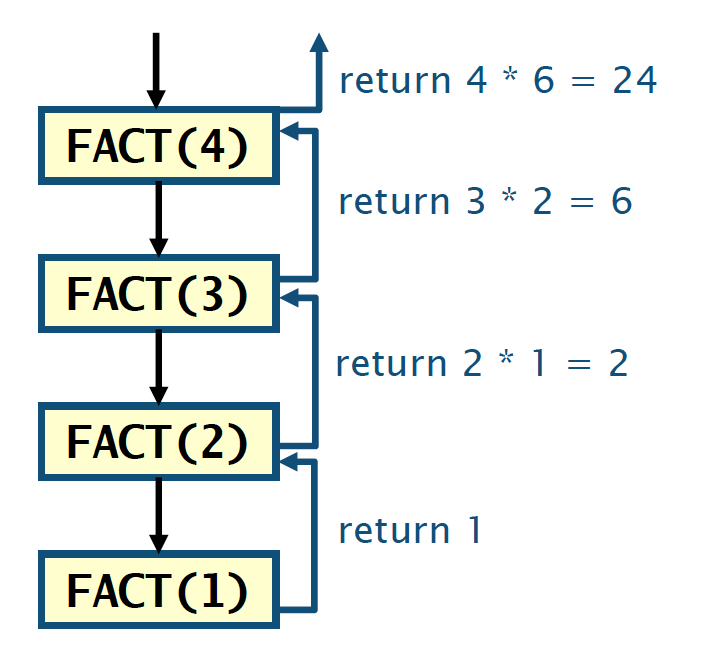
\includegraphics[width=0.4\textwidth]{fact}
}

\subsection{Linear Recursion}

\defn{Linear Recursion}{at most one recursive call with each iteration}

\rem{The space required to keep track of the recursive stack grows linearly with
$n$}

\rem{Useful when we view a problem in terms of a first/last element plus the
remaining set with the same structure (e.g sum array in haskell : \texttt{sum(l) =
head(l) + sum(tail(l))})}

\subsection{Tail Recursion}

\par{Though useful for designing short and elegant algorithms, recursive can
have a high memory cost, since the state of each recursive call must be stored
prior to being returned. This costs can sometimes be diminished by using a
recursive operation and the very last of the algorithm}

\defn{Tail Recursion}{is linear and the recursive call is its very last
operation}

\par{In tail recursive implementations, some variable is modified with each
call. There's no need to wait until the last call, since the updated variable is
immediately passed to the next recursive call. Hence, the state is passed onto
the call chain instead of being saved in memory}

\subsubsection{Recursive $\leftrightarrow$ Iterative}

\par{A common idiom is converting to/from tail recursive to iterative
algorithms. This is achieved by iterating through recursive calls, rather than
calling them explicitily}


\ex{~\cite{hochsteinSO}
\textbf{Recursive}
  \lstinputlisting[firstline=0, lastline=15]{recursionCode.js}
\textbf{Tail Recursive}
  \lstinputlisting[firstline=16, lastline=30]{recursionCode.js} 
\textbf{Iterative}
	\lstinputlisting[firstline=34, lastline=38]{recursionCode.js}
}

\subsection{Binary Recursion}

\defn{Binary Recursion}{when an algorithm makes two recursive calls}

\ex{Fibonacci : FIB(n-1) + FIB(n-2)}

\rem{Highly inefficient. Note how the same computations are made several times
over, in different calls. In the recursion tree there are $O(2^n)$ recursive
calls, i.e exponential complexity~\mymarginpar{recall memoization technique from
1P}}

\section{Algorithm Design Paradigms}

\subsection{Incremental}

\par{The solution of a problem is built one element at a time}

\ex{\vphantom{.\\}
\par{Sort sub array ; pick unvisited node ; add to sorted subarray}

\lstinputlisting[firstline=0, lastline=8]{algCode.py}
}

\subsection{Divide-and-Conquer} 

\par{Recursive algorithm, with 3 steps}

\begin{enumerate}
	\item Divide into smaller subproblems equivalent to the original 
	\item Conquer by solving subproblems recursively
	\item Combine the solutions to the subproblems to give the general solution
\end{enumerate}

\ex{\vphantom{.\\}

\par{\textbf{Merge-Sort} (1) split the array into two subarrays of size
$\frac{n}{2}$ ; (2) scan two smaller arrays simultaneously ; (3) add minimum to
sorted array, incrementing the pointer of the array from where the value was
removed; when fully scanned copy the remaining sub array to main array}
}

 

%\section{Efficient Sorting}

\subsection{Merge Algorithm}

		\defn{Sentinel}{a number which is much larger than any other number in the
		array. It can be represented by \texttt{Integer.MAX\_VALUE}}

		\rem{A more general definition sees sentinel as any value which is interpreted
		as a condition to terminate the algorithm}

		\defn{Stable}{an algorithm which preserves the input order of repeated elements}

		\rem{note that this is only relevant if the repeated elements are somehow
		distinguishable (e.g deck of cards , (rank,value))}

		\defn{Key}{for data being recorded as a tuple of values, the key is the value
		used to sort (e.g (name, surname) , K=S)}

		\defn{Merging Algorithm}{an algorithm which takes two sorted sequences and
		returns a single combined sequence~\cite{merge}}

\subsubsection{Overview}

		\par{The merge algorithm takes an unsorted array and 3 indices, it then splits
		the array into two subarrays and copies each subarray into memory. Finally, it
		iterates over every element of the original array, for each iteration it
		compares the current elements of the 2 subarrays against each other, replacing
		the appropriate value into the original array and increasing the index of the
		subarray by $1$}

\subsubsection{Formal Definition}

\begin{algorithm}[H]
	\DontPrintSemicolon
	\SetAlgoLined\KwData{Array $A$ , indeces $p,q,r$}
	\SetKwFunction{KwFn}{Merge}
	\KwResult{sorted subarray $A[p..r]$}
	\KwFn{A,p,q,r}\\
	$n_1$ := q - p + 1{\tcc*[r]{initialize subarrays' size}}\;
	$n_2$ := r - q\;
	L[0..$n_1$] := A[p..q]{\tcc*[r]{copy to subarrays}}\;
	R[$n_2$..r] := A[q+1..r]\;
	L[$n_1$] := $\infty${\tcc*[r]{add the sentinel values to end of
subarrays}}\;
	R[$n_2$] := $\infty$\;
	i,j := 0\;
	\For{k=p \KwTo r}{\;
	    \uIf{L[i] $\leq$ R[j]}{\;
			A[k] := L[i]\;
			i := i + 1\;
		}
		\uElse{\;
			A[k] := R[j]\;
			j := j + 1\;
		}
	}
		\caption{Merge}
\end{algorithm}

\subsubsection{Properties}

		\begin{itemize}
			\item\textbf{Running Time : } $O(n)$ , since the initialization of
the $L , R$ subarrays takes $O(n)$ and the loop is executed $n$ times and
contains only constant-time operations
			\item\textbf{Stable}
			\item\textbf{Memory Requirements : } $O(n)$ to store $L, R$	
		\end{itemize}

\subsection{Merge-Sort}

\rem{See informal definition in previous section}

\subsubsection{Formal Definition}

	\begin{algorithm}[H]
	\DontPrintSemicolon
	\SetAlgoLined\KwData{Array $A$ , indeces $p,r$}
	\SetKwFunction{KwFn}{Merge-Sort}
	\SetKwFunction{KwFn2}{Merge}
	\KwResult{sorted array $A[p..r]$}
	\KwFn{A,p,r}\\
	\uIf{p < r}{
		q := (p + r) / 2\;
		\KwFn(A,p,q)\;
		\KwFn{A,q+1,r}\;
		\KwFn2{A,p,q,r}\;
	}
	\caption{Merge-Sort Algorithm}
	\end{algorithm}

\subsubsection{Execution \& Properties}

\rem{to sort an array $A$ with $n$ elements, we would call
\texttt{MERGE-SORT(A,0,n-1)}}

\par{Note how the algorithm gives rise to a binary recursive tree, since we
split each subarray into 2 with each iteration until we hit the stopping
condition (single element array). So, the first subarray is entirely sorted,
before the second \texttt{MERGE-SORT} call. The two \ita{half-subarrays} returned
from each call are then merged by calling \texttt{MERGE}. The process is then
repeated in the right branch}

\begin{figure}[H]
	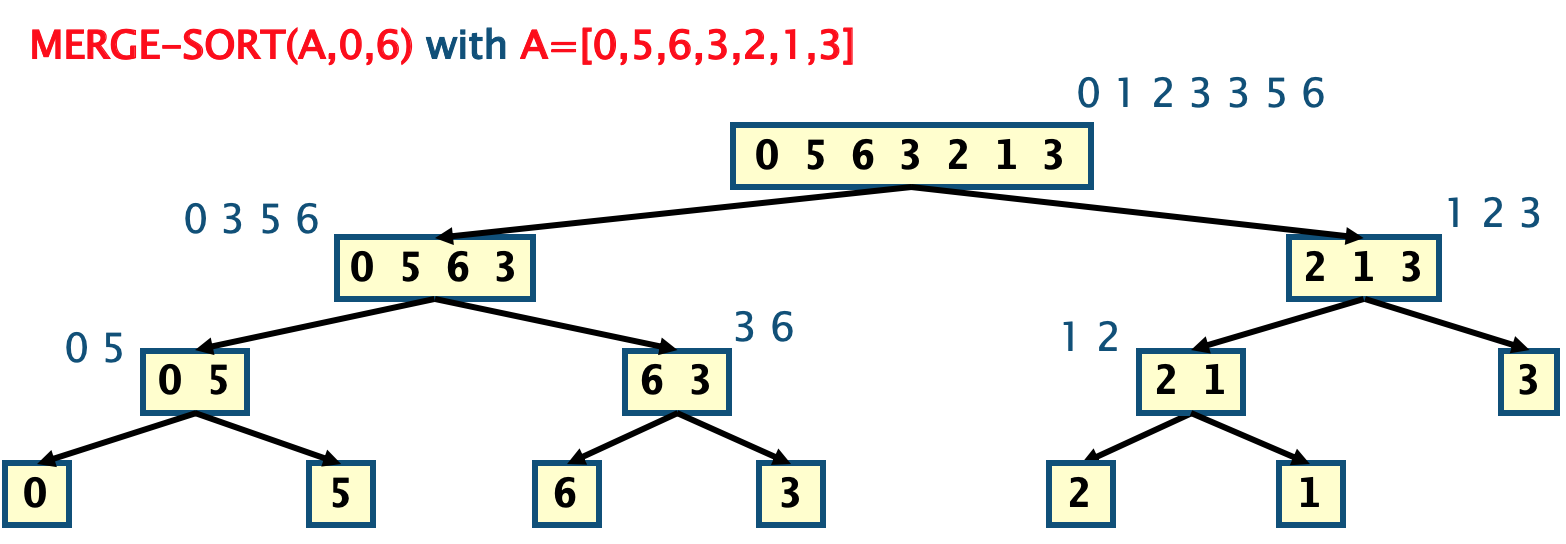
\includegraphics[width=\textwidth]{mergeTree}
\end{figure}

\begin{itemize}
	\item\textbf{Stable}
	\item\textbf{Memory} $O(n)$
	\item\textbf{Running Time} $O(n \log n)$
\end{itemize}

\subsection{Recurrence Equations}


\defn{Recurrence Equation}{describe the overall running time of a problem of
size $n$ in terms of the running time on smaller inputs}
	

\par{Recursive algorithms can be described via \ita{recurrence equations}. Take
$t(n)$ to denote the \ita{worst-case} running time of \texttt{MERGE-SORT(n)},
then we can characterize $t(n)$ by means of an equation where $t(n)$ is
recursively expressed in terms of itself.
}
\par{If \texttt{MERGE-SORT(n)} has running time $T(n)$ then, each recursive call
will \texttt{MERGE-SORT(n/2)} will run on $T(n/2)$ time. Hence, we can define
$T(n)$ recursively as follows}

$$ T(n) = \left\{ 
	\begin{array}{ll}
		b & n \leq 1 \quad \text{(base case)} \\
		2T(n/2) + cn 
	\end{array}
\right.
$$
\subsubsection{Iterative Method}
\par{Though correct, a more informative definition will be one that does not
involve $T(n)$ itself. From its \ita{closed-form} characterization, we can
define it in \ita{big-Oh} terms. We do this, by iterative substitution on the
RHS of the recurrence relation until the base case is reached}
\par{Continuing with the expression above, if we substitute $n$ by $n/2$ in the RHS we
essentially double the children arrays, and we get}

\begin{align*}
	T(n) &= 2(2T((n/2)/2) + c(n/2)) + cn \\
		&= 2^2t(n/2^2) + 2(cn/2) + cn \\
		&= 2^2t(n/2^2) + 2cn
\end{align*}

\par{If we repeat the process, assuming that $n$ is relatively large, then we
find the general pattern}

$$t(n) = 2^it(n/2^i) +  icn$$

\par{In order to determine the base case, we look at the original definition,
and observe that  we need to find $t(n)$ , for $n \leq 1$. Given our general
argument $\frac{n}{2^i}$ we need $2^i = n \iff i = \log n$. Hence, substituting
$i$ by $ \log n$ gives}

\begin{align*}
	t(n) &= 2^{\log n} t(n/2^{\log n}) + cn\log n \\
		&= nt(1) + cn\log n \\
		&= nb + cn\log n
\end{align*}

\par{Lastly, since $b,c$ are constants, we have shown that $t(n)$ is $O(n\log
n)$}

\subsubsection{Master Method}

	\par{There is a general form of recurrence relation that arises in the
analysis of the divide-and-conquer algorithms}

$$T(n) = aT(n/b) + f(n) \qquad a , b \geq 1$$

	\par{Then, for $f(n) = \Theta(n^c)$ , the solution will be one of the
following 3 cases}

	\begin{enumerate}
		\item $
\mathrm{c}<\log _{\mathrm{b}} \mathrm{a} \text { then } \mathrm{T}(\mathrm{n})=\Theta\left(n^{\log _{b} a}\right)
$
		\item $
\mathrm{c}=\log _{\mathrm{b}} \mathrm{a} \text { then } \mathrm{T}(\mathrm{n})=\Theta(\mathrm{n} \leq \log \mathrm{n})
$
		\item $
\mathrm{c}>\log _{\mathrm{b} 2} \mathrm{a} \text { then } \mathrm{T}(\mathrm{n})=\Theta(\mathrm{f}(\mathrm{n}))
$
	\end{enumerate}

\par{For \texttt{MERGE-SORT}, we have $a=2 , b=2 , f(n) = \Theta(n) , c = 1$ .
Hence, the solution is given by case $2$ , $\Theta(n^c \log n) = \Theta(n \log
n)$}

\subsubsection{Tree Method}

\rem{See lecture 5 slides 52-60}


\subsection{Quicksort}


\section{Abstract Data Types}

\defn{ADT}{ is a mathematical model of a data structure that specifies the type of data stored, the operations supported on them, and the types of parameters of the operations}

\par{ADTs are abstractions of the structure of data from the data itself, they define behaviour and state, a contract whose concrete instances must follow. When implemented in code we do so via \ita{data structures}. For example, a \texttt{List} can be implemented as an \texttt{array}}

\rem{In \texttt{Java} you can think in terms of \texttt{Interfaces} and \texttt{Classes}}

		\subsection{Stack}

				\defn{Stack}{is a collection of objects that are inserted and removed following the \ita{LIFO} principle}

				\rem{Web browsers' histories use stacks, and undo sequences in most other software work in a similar manner}
  
		\subsubsection{Operations}

				\begin{itemize} 
								\item Essential Update Methods 
						\begin{enumerate}
								\item push
								\item pop
						\end{enumerate}
				\end{itemize}
				\begin{itemize}
								\item Accessor Methods
						\begin{enumerate}
								\item top : "pop" without removing
								\item size
								\item isEmpty
						\end{enumerate}
				\end{itemize}

		\subsubsection{Implementation - Array}

				\par{The array implementation of a stack is simple and efficient \ita{if} one has a good idea , in advance , of the number of elements it will contain. Then, given $n,t$ where $n$ represents the size of the stack and $t$ is a cursor var which keeps track of the index of top element, one adds elements from [0...n-1=t]}

		\rem{by convention , $ S = \emptyset \iff t = -1 $}

		\defn{Stack Overflow}{ push() into full stack}
		\defn{Stack Underflow}{ pop() empty stack}

		\subsubsection{Operations}
			\begin{algorithm}[H]
				\DontPrintSemicolon
				\SetAlgoLined\KwData{Stack $S$}
				\SetKwFunction{KwFn}{STACK-EMPTY}
				\KwResult{true, false}
				\KwFn{S}\\
				\Indp\Return S.top = -1

				\caption{isEmpty}

			\end{algorithm}

			\begin{algorithm}[H]
				\DontPrintSemicolon
				\SetAlgoLined\KwData{Stack $S$ , $x$}
				\SetKwFunction{KwFn}{PUSH}
				\KwFn{S,$x$}{\\
				\Indp S.top := S.top + 1 \;
				\Indp S[S.top] := x 
				}
				\caption{Push}

			\end{algorithm}

		\begin{algorithm}[H]
				\DontPrintSemicolon
				\SetAlgoLined\KwData{Stack $S$}
				\SetKwFunction{KwFn}{POP}
				\KwResult{"underflow", S[S.top + 1]}
				\KwFn{S}\\
				\uIf{STACK-EMPTY(S)}
					{return "underflow"}
				\uElse{
					S.top := S.top - 1 \;
					\Return S[S.top + 1]
					}

				\caption{Pop}

			\end{algorithm}

		\subsubsection{Analysis}

				\par{Each method executes a constant number of statements involving
arithmetic operations, comparisons, and assignments, or calls to size and isEmpty,
which both run in constant time, i.e they're all $O(1)$, and memory is $O(n)$}

		\subsubsection{Implementation - Dynamic Array}

				\par{One can overcome the fixed size constraint by adding a \texttt{RESIZE} operation, allowing the array to both shrink and grow.}
				\par{Simple implementations are doubling its size when full, and half it when it is one quarter full. So, when an overflow is detected the following happens:}
				\begin{enumerate}
						\item Allocate a new array $S'$ with larger capacity
						\item Set $S'[k] = S[k] , k = 0 , \dots , n-1$
						\item Set $S = S'$
				\end{enumerate}

		\subsubsection{Operations}
						\begin{algorithm}[H]
				\DontPrintSemicolon
				\SetAlgoLined\KwData{Stack $S$ , new capacity $n'$}
				\SetKwFunction{KwFn}{RESIZE}
				\KwFn{S, n'}\\
				\Indp new S’[0..n’-1] \;
				\For{i = 0 to S.top}
					{S’[i] := S[i]}
				S := S'
				\caption{Resize}

			\end{algorithm}

			\begin{algorithm}[H]
				\DontPrintSemicolon
				\SetAlgoLined\KwData{Stack $S$ , $x$}
				\SetKwFunction{KwFn}{PUSH}
				\KwFn{S,$x$}{\\
				\uIf{S.top = n -1}
					{RESIZE(S, 2*n) {\tcc*[r]{double array if full}}
					}
				S.top := S.top + 1 \;
				S[S.top] := x 
				}
				\caption{Push}

			\end{algorithm}

		\begin{algorithm}[H]
				\DontPrintSemicolon
				\SetAlgoLined\KwData{Stack $S$}
				\SetKwFunction{KwFn}{POP}
				\KwResult{"underflow", S[S.top + 1]}
				\KwFn{S}\\
				\uIf{STACK-EMPTY(S)}
					{return "underflow"}
				\uElse{
					x := S[S.top]\;
					S.top := S.top - 1 \;
					\If{S.top > 0 and S.top = n/4}
						{RESIZE(S,n/2){\tcc*[r]{half array if 1/4 full}}
					}
					\Return S[S.top + 1]
				}

				\caption{Pop}

			\end{algorithm}

		\subsubsection{Analysis}
						\begin{itemize}
								\item[] Memory : $O(kn)$
								\item[] \mymarginpar{see L.8.35 for amortised analysis}Running Time : O(n) , since when expanding by a constant proportion each insertion takes \ita{amortised} constant time
						\end{itemize}

		\subsubsection{Implementation - Linked List}
				\par{Let \texttt{l.head := S.top} , then \texttt{PUSH = INSERT@Head} , \texttt{POP = DEL@Head} and by keeping track of size with \texttt{S.size} we can perform \texttt{SIZE} at constant time}

		\subsubsection{Operations}

			\begin{algorithm}[H]
				\DontPrintSemicolon
				\SetAlgoLined\KwData{Stack $S$ , $x$}
				\SetKwFunction{KwFn}{PUSH}
				\KwFn{S,$x$}{\\
				\Indp x.next := S.top {\tcc*[r]{S.top == L.head}} \;
				\Indp S[S.top] := x 
				}
				\caption{Push}

			\end{algorithm}

		\begin{algorithm}[H]
				\DontPrintSemicolon
				\SetAlgoLined\KwData{Stack $S$}
				\SetKwFunction{KwFn}{POP}
				\KwResult{"underflow", x}
				\KwFn{S}\\
				\uIf{S.top != NILL}
					{x := S.top \;
					 S.top := S.top.next \;
					 \Return x
					}
				\uElse{
					\Return "underflow"
					}

				\caption{Pop}
		\end{algorithm}
	
		\subsubsection{Analysis}
						\begin{itemize}
								\item[] Memory : $O(n)$
								\item[] Running Time : O(1)
						\end{itemize}


\subsection{Queue}

		\defn{Queue}{ is a collection of objects which are inserted and deleted following the \ita{FIFO} principle}

		\rem{sharing services (e.g printer) , waiting lists, multitasking}

		\subsubsection{Operations}
				\begin{itemize}
						\item Essential Update Methods
						\begin{enumerate}
								\item enqueue
								\item dequeue
						\end{enumerate}
				\end{itemize}
				\begin{itemize}
						\item Accessor Methods
						\begin{enumerate}
								\item first
								\item size
								\item isEmpty
						\end{enumerate}
				\end{itemize}
				
		\subsubsection{Array Implementation}
				
				\par{Using a \ita{wrap-around} array, let \texttt{Q.head , Q.tail} represent the head index and the \texttt{tail+1} index respectively. One leaves \texttt{Q[Q.tail]} empty to insert new values, and delete from \texttt{Q[Q.head]}}

		\subsubsection{Operations}

				%% lstlisting %%

		\subsubsection{analysis}
			\begin{itemize}
				\item[] Memory : $O(n)$
				\item[] Running Time : $O(1)$
			\end{itemize}	

		\rem{Queue max-size defined \ita{a priori}}

		\subsection{Implementation : Linked List}

		\par{Take \texttt{L.head == Q.head} and \texttt{L.tail == Q.tail} then, for a queue to align its front with the front of the list, and similarly their back then \texttt{ENQUEUE, DEQUEUE} are implemented via \texttt{INSERT@TAIL, DELETE@HEAD} respectively}

		\subsection{Analysis}
				\begin{itemize}
						\item[] Running Time \mymarginpar{\texttt{SIZE} will need to keep track of \texttt{Q.tail}}: $O(1)$
				\end{itemize}

		\rem{Doubly-linked lists offer the same running time, but at a higher memory cost}

\section{Double Ended Queue}

		\par{Structures similar to queues which support data insertion and deletion at both the start and end}

		\rem{\ita{deque} read as \ita{"deck"}}

		\subsection{Operations}
			\begin{itemize}
						\item[] Update Methods
				\begin{enumerate}
						\item addFirst
						\item addLast
						\item delFirst
						\item delLast
				\end{enumerate}
						\item[] Accessor Methods
				\begin{enumerate}
						\item first
						\item last
						\item size
						\item isEmpty
				\end{enumerate}
			\end{itemize}
		
		\subsection{Analysis}
				\par{All operations run on $O(1)$, and depending on their implementation $O(N)$ for an array of size $N$ and $O(n)$ , where $n < N$ is the actual number of elements in a doubly linked list}



\section{List}

		\par{The ADTs presented above could all be implemented using either an array or a linked list, due to fact that they represent a \ita{linearly ordered} sequence of elements. The \texttt{List} however provides more general support for manipulating a sequence of countable elements at arbitrary positions, hence an efficient implementation with either an array or linked list is challenging}

		\rem{fundamental data type in most functional languages}

		\subsection{operations}
				\begin{enumerate}
						\item[] GET(L,i)
						\item[] SET(L,i,x) : add x at i, return replaced 
						\item[] ADD(L,x)
						\item[] ADD-AT(L,i,x) : add x at i, shift right
						\item[] REMOVE(L,i) : remove and shift left
						\item[] SIZE()
						\item[] isEmpty()
						\item[] APPEND(L1,L2)
				\end{enumerate}


		\subsection{Analysis}
												\begin{table}[]
								\begin{tabular}{lcccc}
								\cline{2-5}
								\multicolumn{1}{l|}{}                        & \multicolumn{1}{c|}{\textbf{GET/SET (Indexing)}} & \multicolumn{1}{c|}{\textbf{ADD}} & \multicolumn{1}{c|}{\textbf{ADD-AT/REMOVE}} & \multicolumn{1}{c|}{\textbf{APPEND}}  \\ \hline
								\multicolumn{1}{|l|}{\textbf{Dynamic Array}} & \multicolumn{1}{c|}{$O(1)$}                      & \multicolumn{1}{c|}{$O(n)$}       & \multicolumn{1}{c|}{$O(n)$}                 & \multicolumn{1}{c|}{\$O(n\_1 + n\_2)} \\ \hline
								\multicolumn{1}{|l|}{\textbf{Linked List}}   & \multicolumn{1}{c|}{$O(n)$}                      & \multicolumn{1}{c|}{$O(1)$}       & \multicolumn{1}{c|}{$O(n)$}                 & \multicolumn{1}{c|}{$O(1)$}           \\ \hline
																														 & \multicolumn{1}{l}{}                             & \multicolumn{1}{l}{}              & \multicolumn{1}{l}{}                        & \multicolumn{1}{l}{}                 
								\end{tabular}
								\end{table}

%%%%%%%%%%%%%%  BIBLIOGRAPHY  %%%%%%%%%%%%%%%%%%%
\newpage
\nocite{*}
\printbibliography

%%%%%%%%%%%%%%%%%%%%%%%%%%%%%%%%%%%%%%%%%%

\end{document}
